\documentclass[11pt]{article}
\usepackage[a4paper,margin=2.2cm]{geometry}
\usepackage[T1]{fontenc}
\usepackage{lmodern}
\usepackage{microtype}
\usepackage{amsmath,amssymb}
\usepackage{booktabs}
\usepackage{graphicx}
\usepackage{caption}
\usepackage{float}
\usepackage[section]{placeins}
\usepackage{enumitem}
\setlist{nosep,leftmargin=*,topsep=2pt}
\usepackage[authoryear,round]{natbib}
\usepackage[colorlinks=true,linkcolor=black,citecolor=black,urlcolor=blue]{hyperref}
\captionsetup{font=small,labelfont=bf,skip=4pt}
\setlength{\parskip}{3pt}
\graphicspath{{../output/figures/}}
\newcommand{\NTargets}{127,454}
\newcommand{\NCommon}{95,732}
\newcommand{\NFirmsCommon}{2,751}
\newcommand{\PctCommon}{75.1}
\newcommand{\NTrim}{94,774}
\newcommand{\NFirmsFL}{2,124}
\newcommand{\NYears}{17}
\newcommand{\NQuarters}{65}
\newcommand{\MAErw}{0.0860}
\newcommand{\RMSErw}{0.4791}
\newcommand{\MAExgb}{0.0681}
\newcommand{\RMSExgb}{0.3906}
\newcommand{\dMAExgb}{20.8}
\newcommand{\dRMSExgb}{18.5}
\newcommand{\dMAErwd}{$-$8.4}
\newcommand{\dRMSErwd}{$-$4.5}
\newcommand{\dMAEfoster}{$-$14.6}
\newcommand{\dRMSEfoster}{$-$29.6}
\newcommand{\dMAEpooled}{$-$7.5}
\newcommand{\dRMSEpooled}{$-$6.3}
\newcommand{\dMAExgbTrim}{17.8}
\newcommand{\dRMSExgbTrim}{17.7}
\newcommand{\dMAEfosterTrim}{$-$13.4}
\newcommand{\dRMSEfosterTrim}{$-$10.0}
\newcommand{\dMAErwdTrim}{$-$9.6}
\newcommand{\dRMSErwdTrim}{$-$6.6}
\newcommand{\dsMAExgb}{14.0}
\newcommand{\MedAErw}{0.0250}
\newcommand{\MedAExgb}{0.0225}
\newcommand{\tMAExgb}{7.79}
\newcommand{\tRMSExgb}{1.77}
\newcommand{\tDMMAExgb}{8.79}
\newcommand{\tDMRMSExgb}{1.74}
\newcommand{\tRMSExgbTrim}{9.07}
\newcommand{\tDMRMSExgbTrim}{10.01}
\newcommand{\QbetterMAExgb}{95.4}
\newcommand{\QbetterRMSExgbTrim}{96.9}
\newcommand{\YearsBestMAExgb}{17}
\newcommand{\YearsBestRMSExgb}{16}
\newcommand{\MinAnnualdMAExgb}{11.6}
\newcommand{\MaxAnnualdMAExgb}{35.6}
\newcommand{\FirmBetterxgb}{87.7}
\newcommand{\FirmBetterRMSExgb}{86.8}
\newcommand{\FirmBetterrwd}{17.7}
\newcommand{\FirmBetterfoster}{21.3}
\newcommand{\FirmMedxgb}{18.7}
\newcommand{\TopTenSharexgb}{49.3}
\newcommand{\ExclTopFivexgb}{18.2}
\newcommand{\ExclTopTenxgb}{16.4}
\newcommand{\ExclHardxgb}{19.8}
\newcommand{\PhiFirmMed}{0.08}
\newcommand{\PhiPooledMed}{0.12}
\newcommand{\PhiCapped}{1.3}
\newcommand{\dMAExgbQoneNP}{7.5}
\newcommand{\dMAExgbQoneP}{13.6}
\newcommand{\dMAEfosterQoneP}{$-$56.4}
\newcommand{\SameDayLate}{43}
\newcommand{\SameDayEarly}{4}
\newcommand{\XcheckN}{74,390}
\newcommand{\XcheckPct}{100.0}
\newcommand{\LookaheadN}{12,303}
\newcommand{\TopImp}{loss\_l4}
\newcommand{\TopImpShare}{19.1}
\newcommand{\GainTopOnePctObs}{43.0}
\newcommand{\GainTopTenPctObs}{95.0}
\newcommand{\XGBfits}{129}
\newcommand{\XGBbatches}{232}
\newcommand{\PeriodOne}{21.0}
\newcommand{\PeriodTwo}{22.7}
\newcommand{\PeriodThree}{20.2}


\title{Out-of-Sample Forecasts of Quarterly EPS for Chinese A-Shares:\\
Seasonal Random Walk, Foster, and XGBoost, 2005--2021}
\author{Forecast-accuracy report for the PEAD / gambler's-fallacy project}
\date{October 2026}

\begin{document}
\maketitle

\begin{abstract}
\noindent Standardized unexpected earnings (SUE) are only as good as the expectation model behind them. Using
\NTargets{} Shanghai and Shenzhen firm-quarter announcements from FY2005Q1 to FY2021Q1, I compare four expectation
models for quarterly EPS in a strictly out-of-sample design. The models are the seasonal random walk (SRW), the SRW with drift,
a Foster (1977) seasonal autoregression, and a pooled XGBoost model. All share a 12-quarter rolling window and the
information set available the day before each announcement. On the common sample of \NCommon{} forecasts, XGBoost
lowers MAE by \dMAExgb\% and RMSE by \dRMSExgb\% relative to the SRW. It is the most accurate model by MAE in every
year and beats the SRW for \FirmBetterxgb\% of firms. The firm-specific drift and Foster models are \emph{less}
accurate than the SRW: short Chinese EPS histories cannot estimate the extra parameters precisely enough.
\end{abstract}

\section{Introduction and motivation}

Post-earnings-announcement drift (PEAD) is measured by sorting firms on an earnings surprise, so the surprise has
to approximate what investors expected. The workhorse measure scales the seasonal change in quarterly EPS,
$UE_{i,q}=EPS_{i,q}-EPS_{i,q-4}$, by its historical standard deviation. That is, it uses a seasonal random walk as the
expectation \citep{bernard1990}. \citet{foster1977} showed that seasonal differences of quarterly earnings are
positively autocorrelated, so a seasonal autoregression can beat the pure random walk. \citet{bernard1990} built their
PEAD evidence on exactly this autocorrelation structure. If a better expectation model is available, the SRW leaves
predictable components in ``unexpected'' earnings. Surprise sorts then become noisier, and PEAD estimates may be
attenuated or mis-attributed.

Two recent strands make the choice of expectation model more pressing. First, machine-learning (ML) forecasts can be
more accurate than traditional benchmarks, but conclusions about their superiority depend on a clean, look-ahead-free
training design and on what the forecast is meant to represent \citep{zhang2025}. Second, \citet{campbell2026} stress
that the most accurate statistical forecast is not automatically the market's expectation. Which model to use depends
on whether a study needs an accurate forecast or a proxy for investors' beliefs. In the same spirit,
\citet{pagach2020} revisit the maintained assumption that analysts dominate time-series models for quarterly earnings.
For Chinese A-shares, where analyst coverage was thin for much of the sample, time-series and ML forecasts are the
natural candidates.

This report is limited to forecast accuracy. It asks which of four models best predicts quarterly EPS out of
sample, how stable the ranking is over time, and whether the gains are broad-based across firms. The saved forecasts
give alternative surprises $UE^{(m)}_{i,q}=EPS_{i,q}-\widehat{EPS}^{(m)}_{i,q}$ for the PEAD analysis.

\section{Data and methodology}

\paragraph{Data reconstruction.} The only input is the monthly Shanghai--Shenzhen panel (515,915 firm-months, 3,594 firms).
Its quarterly fields are stored by calendar quarter rather than by information arrival. Each calendar year's rows carry
that fiscal year's four EPS values, and \texttt{eps\_q$k$}/\texttt{date\_q$k$} sit in the three rows of calendar quarter
$k$. A January row therefore already contains Q1 EPS that is published in April. I rebuild the data at the
firm--fiscal-quarter level and treat a value as known only from its publication date \texttt{date\_q$k$}. Three checks
shape this step:
\begin{itemize}
\item \emph{Standalone values.} EPS is standalone quarterly, not year-to-date: the median ratio of Q2 (Q4) to Q1 EPS is
about 1.3 (1.2--1.6), and only 5--15\% of profitable firm-years rise monotonically through the year.
\item \emph{Adjusted values.} EPS is retroactively adjusted for later bonus issues, which keeps year-over-year changes on
a common share basis.
\item \emph{Unreliable dates.} Publication dates before FY2004 are mostly vendor backfill dates (Nov 2003 -- Jan 2004).
They are used as given, which is conservative. Values with missing or impossible dates are never used, and identical
values repeated across fiscal years are dropped.
\end{itemize}
Evaluation targets are all firm-quarters of FY2005Q1--FY2021Q1 (FY2021: Q1 only, since the panel ends in May 2021)
announced within 365 days of quarter end. Table~\ref{tab:sample} reports coverage.

\paragraph{Information order.} The fiscal order of quarters is not the order in which information arrives. Annual (Q4)
and Q1 reports share an April 30 deadline, and the prior-year annual report was released on the \emph{same day} as
the Q1 report for \SameDayEarly\% of Q1 announcements in 2005--2012 but \SameDayLate\% in 2019--2021
(notebook Figure~0). For these targets $EPS_{q-1}$ is not public at the forecast origin, and every model below is
built to respect this.

\paragraph{Models.} Let $\Delta_4 EPS_s=EPS_s-EPS_{s-4}$.
\begin{itemize}
\item[M1] \emph{SRW:} $\widehat{EPS}_q=EPS_{q-4}$.
\item[M2] \emph{SRW with drift:} $\widehat{EPS}_q=EPS_{q-4}+\hat\mu_i$, where $\hat\mu_i$ is the mean of the firm's
$\Delta_4 EPS_s$ in the estimation window ($\geq4$ changes required).
\item[M3] \emph{Foster seasonal AR(1):} firm-specific OLS of $\Delta_4 EPS_s=\alpha_i+\phi_i\,\Delta_4 EPS_{s-1}+\varepsilon_s$
($\geq8$ pairs required, $\hat\phi_i$ capped to $[-1,1]$). The forecast is
$EPS_{q-4}+\hat\alpha_i+\hat\phi_i\,\Delta_4 EPS_{q-1}$. If $EPS_{q-1}$ is not yet public, the iterated two-step form
$EPS_{q-4}+\hat\alpha_i(1+\hat\phi_i)+\hat\phi_i^2\,\Delta_4 EPS_{q-2}$ is used. As a robustness check, $\phi$ is pooled
across firms (within-firm estimator on firm-scaled, winsorized pairs), keeping a firm-specific intercept.
\item[M4] \emph{XGBoost} \citep{chen2016}: one model pooled across firms, predicting
$\Delta_4 EPS_q$ scaled by the firm's mean $|EPS|$ over its last eight known quarters. Features: scaled EPS lags 1--8
and 12, YoY-change lags 1--4, window mean/median/SD of YoY changes, EPS volatility, trailing-four-quarter growth,
loss frequency and a lag-4 loss indicator, the log EPS scale, history length, the fiscal quarter, and the number of
quarters to the latest public EPS. Lags not yet public are left missing. The grid is deliberately small (depth 2--4,
learning rate 0.05, subsampling 0.8, early stopping).
\end{itemize}

\paragraph{Rolling out-of-sample design.} All models use the same origin, horizon and window:
\begin{itemize}
\item \emph{Origin and horizon.} The forecast is made the day before the target's announcement date $A$. Inputs are
restricted to EPS announced strictly before $A$, and the horizon is the next announcement.
\item \emph{Window.} Parameters are estimated on training targets in fiscal quarters $q-12,\ldots,q-1$ (a 12-quarter
rolling window) that were announced before the first day of $A$'s month. This common estimation cutoff lets XGBoost be
refit monthly (\XGBfits{} fits for \XGBbatches{} re-estimation batches). Twelve quarters is also the longest window
feasible from 2005, since Q1 and Q3 data are sparse before FY2002.
\item \emph{XGBoost training and tuning.} XGBoost training rows are built ``as of'' their own announcement dates, and the
training target is winsorized with training-set quantiles. Hyperparameters are re-tuned each January using only data
available then: training targets announced in the previous year form the validation set, and earlier ones the fit set.
\end{itemize}

Figure~\ref{fig:rolling-design} illustrates the design. ``Rolling'' means that, when the target advances by one
fiscal quarter, the oldest quarter leaves the estimation window and the newest one enters. ``Out of sample'' means
that the target's realized EPS is withheld until after its forecast has been saved. The two cutoffs serve different
purposes: model parameters use outcomes public before the announcement month begins, while the forecast's inputs
can incorporate earnings released later in that month, up to the day before the target announcement.

\begin{figure}[H]
\centering
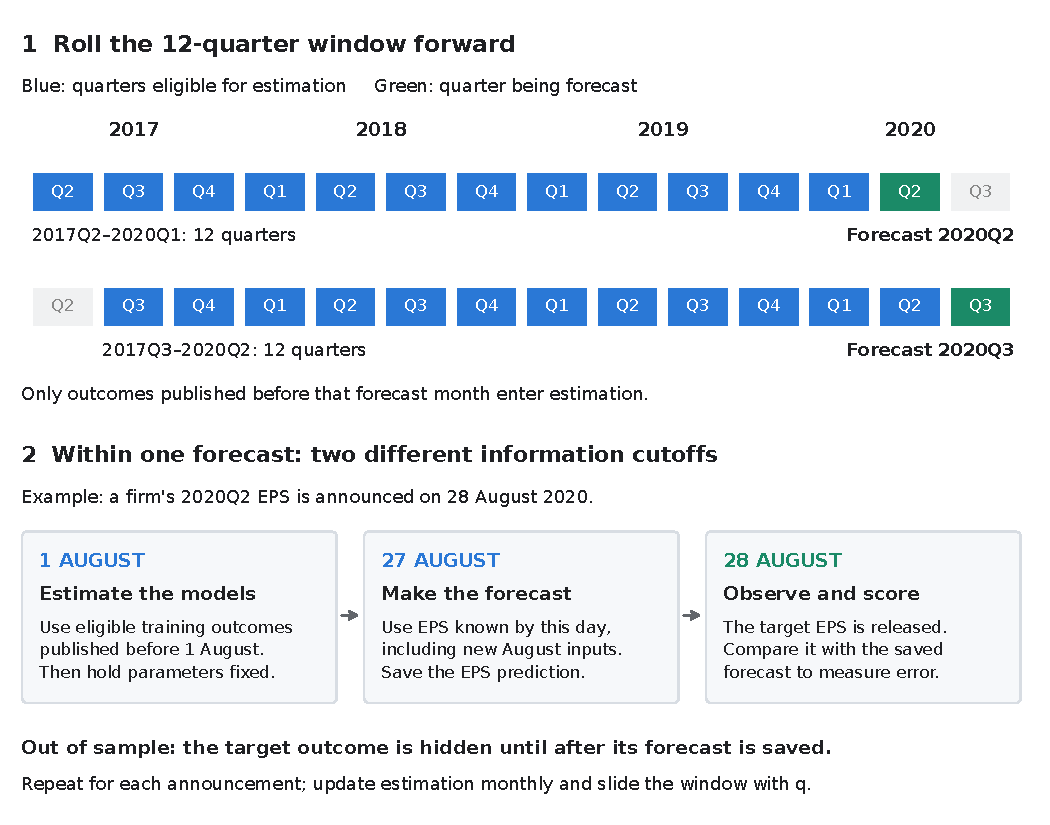
\includegraphics[width=\linewidth]{fig_rolling_oos_design.pdf}
\caption{Rolling out-of-sample forecasting: an illustrative example. For a 2020Q2 target announced on 28 August,
the eligible estimation quarters are 2017Q2--2020Q1, and only training outcomes published before 1 August are used.
The forecast uses inputs public before 28 August. For a 2020Q3 target, the window advances to 2017Q3--2020Q2.
Blue quarters indicate eligibility, not guaranteed availability. Parameter estimation applies to drift, Foster and
XGBoost; the seasonal random walk simply uses the same quarter's EPS from the previous year.}
\label{fig:rolling-design}
\end{figure}

\paragraph{Leakage controls.} The notebook verifies four things:
\begin{enumerate}
\item every input and estimation datum predates its cutoff;
\item a slow, label-based re-implementation reproduces M1--M3;
\item an end-to-end perturbation test holds: replacing all EPS announced after 1 January 2008 with random numbers
leaves all \LookaheadN{} earlier forecasts bit-identical, including XGBoost tuning and refits, while a deliberately
leaky variant fails the same test;
\item the M1 surprises reproduce the existing Stata $UE$ measure for \XcheckPct\% of \XcheckN{} matched announcements.
\end{enumerate}

\paragraph{Evaluation.} Accuracy is measured by MAE and RMSE in CNY per (adjusted) share on the identical common sample
where all four models are available. Improvements are $\%\Delta MAE_m=100(1-MAE_m/MAE_{SRW})$, and likewise for RMSE.
Paired tests use the per-forecast loss differential $d=L(e_{SRW})-L(e_m)$. They report (i) $t$-statistics with
standard errors clustered by firm and fiscal quarter \citep{cameron2011,thompson2011}, and (ii) Diebold--Mariano
statistics on the quarterly mean differential with Newey--West errors \citep{diebold1995,newey1987}.

\begin{table}[!htbp]
\centering\small
\caption{Sample construction and model availability. A target is a firm-quarter announcement in FY2005Q1--FY2021Q1.
M3's minimum of eight Foster pairs is the binding requirement for the common sample.}
\label{tab:sample}
\begin{tabular}{lrrrl}
\toprule
& Firm-quarters & \% of targets & Firms & First forecast \\
\midrule
\multicolumn{5}{l}{\emph{Panel A: comparison period, FY2005Q1--FY2021Q1}} \\
Targets (FY2005Q1--FY2021Q1) & 127,454 & 100.0 & 3,383 &  \\
M1 SRW: $EPS_{q-4}$ public before $A$ & 117,902 & 92.5 & 3,120 &  \\
M2 SRW + drift: $\geq$4 YoY changes & 109,129 & 85.6 & 2,970 &  \\
M3 Foster: $\geq$8 pairs & 95,732 & 75.1 & 2,751 &  \\
M4 XGBoost: $\geq$1,000 training rows & 117,902 & 92.5 & 3,120 &  \\
Foster, pooled $\phi$: $\geq$4 pairs & 105,786 & 83.0 & 2,923 &  \\
Common sample (M1--M4 all available) & 95,732 & 75.1 & 2,751 &  \\
Firms with $\geq$12 common-sample forecasts & 92,584 & 72.6 & 2,124 &  \\
\midrule
\multicolumn{5}{l}{\emph{Panel B: full forecast period (each model as early as its data allow)}} \\
Targets (FY1994Q1--FY2021Q1) & 137,116 & 100.0 & 3,397 &  \\
M1 SRW: $EPS_{q-4}$ public before $A$ & 123,092 & 89.8 & 3,129 & 1996Q2 \\
M2 SRW + drift: $\geq$4 YoY changes & 113,106 & 82.5 & 2,977 & 2002Q2 \\
M3 Foster: $\geq$8 pairs & 96,091 & 70.1 & 2,751 & 2003Q4 \\
M4 XGBoost: $\geq$1,000 training rows & 121,496 & 88.6 & 3,129 & 2004Q1 \\
Foster, pooled $\phi$: $\geq$4 pairs & 108,424 & 79.1 & 2,928 & 2003Q3 \\
\bottomrule
\end{tabular}

\end{table}

\section{Overall results}

Table~\ref{tab:overall} reports the main comparison. XGBoost is the only model that beats the SRW. Its MAE of
\MAExgb{} against \MAErw{} is a \dMAExgb\% improvement, and its RMSE improvement is \dRMSExgb\%. The improvement is
also visible in the median absolute error (\MedAExgb{} vs.\ \MedAErw{}) and in scale-free errors (\dsMAExgb\%). The
added complexity of the parametric models does not pay off. Drift raises MAE by \mbox{\dMAErwd\%}, and firm-specific
Foster by \mbox{\dMAEfoster\%}. Even with $\phi$ pooled across firms, Foster stays below the SRW
(\mbox{\dMAEpooled\%}). The estimated persistence of seasonal differences is low (median firm $\hat\phi=\PhiFirmMed$,
median pooled $\phi=\PhiPooledMed$), so estimation noise in $\hat\alpha_i$ and $\hat\phi_i$ outweighs the small
predictable component.

\begin{table}[!htbp]
\centering\small
\caption{Forecast accuracy. MAE, RMSE and MedAE are in CNY per share. $\%\Delta$ is the improvement relative to the
SRW (positive = better); sMAE scales each absolute error by the firm's historical EPS scale. Panel A uses only
observations with forecasts from all four models. Panel B removes the 1\% of these observations with the largest
absolute error of \emph{any} model. Panel C uses each model's full available sample, without trimming or requiring
forecasts from the other models; its last column reports the observation count $N$, replacing $\%\Delta$sMAE.
Each Panel C improvement compares the model with the SRW evaluated on that model's own sample, so error levels
across rows need not refer to identical observations; Panel A provides the common-sample comparison.
Stars: significance of the mean loss differential,
two-way clustered by firm and fiscal quarter (*** 1\%, ** 5\%, * 10\%).}
\label{tab:overall}
\resizebox{\textwidth}{!}{\begin{tabular}{lrrrrrr}
\toprule
& MAE & RMSE & \%$\Delta$MAE & \%$\Delta$RMSE & MedAE & \%$\Delta$sMAE \\
\midrule
\multicolumn{7}{l}{\emph{Panel A: common sample (N = 95,732)}} \\
SRW & 0.0860 & 0.4791 & -- & -- & 0.0250 & -- \\
SRW + drift & 0.0933 & 0.5006 & $-$8.4*** & $-$4.5* & 0.0287 & $-$9.5 \\
Foster & 0.0986 & 0.6211 & $-$14.6*** & $-$29.6 & 0.0293 & $-$11.8 \\
XGBoost & 0.0681 & 0.3906 & 20.8*** & 18.5* & 0.0225 & 14.0 \\
\midrule
\multicolumn{7}{l}{\emph{Panel B: trimmed common sample (N = 94,774)}} \\
SRW & 0.0641 & 0.1328 & -- & -- & 0.0250 & -- \\
SRW + drift & 0.0703 & 0.1415 & $-$9.6*** & $-$6.6*** & 0.0282 & $-$10.4 \\
Foster & 0.0727 & 0.1460 & $-$13.4*** & $-$10.0*** & 0.0288 & $-$12.8 \\
XGBoost & 0.0527 & 0.1093 & 17.8*** & 17.7*** & 0.0221 & 14.3 \\
\midrule
\multicolumn{7}{l}{\emph{Panel C: model-specific samples (each vs.\ SRW on the same forecasts; last column = N)}} \\
SRW & 0.0810 & 0.4411 & -- & -- & 0.0240 & 117,902 \\
SRW + drift & 0.0906 & 0.4761 & $-$8.6 & $-$4.6 & 0.0280 & 109,129 \\
Foster & 0.0986 & 0.6211 & $-$14.6 & $-$29.6 & 0.0293 & 95,732 \\
XGBoost & 0.0648 & 0.3598 & 20.1 & 18.4 & 0.0216 & 117,902 \\
\midrule
\multicolumn{7}{l}{\emph{Panel D: robustness, Foster with pooled $\phi$ (common sample)}} \\
Foster, pooled $\phi$ & 0.0925 & 0.5091 & $-$7.5 & $-$6.3 & 0.0282 & $-$8.0 \\
\bottomrule
\end{tabular}
}
\end{table}

\paragraph{Extreme errors.} Full-sample RMSE is dominated by a handful of implausible EPS values. For example, one
firm (ANTONG HOLDINGS) reports quarterly EPS of 27.8, 36.5 and $-64.1$ CNY in 2016, which produces the six largest
Foster errors. Accordingly, XGBoost's RMSE gain is only marginally significant in the full sample
($t=\tRMSExgb$; Table~\ref{tab:tests}). After symmetric trimming of the 1\% largest errors (Panel B), XGBoost improves
MAE by \dMAExgbTrim\% and RMSE by \dRMSExgbTrim\%, and both differentials are highly significant ($t=\tRMSExgbTrim$
for squared loss). XGBoost has the lower average absolute loss in \QbetterMAExgb\% of the \NQuarters{} fiscal
quarters. The gain is concentrated where surprises are large. Forecasts in the top decile of $|\Delta_4 EPS|$ account
for \GainTopTenPctObs\% of XGBoost's net MAE reduction, while for near-zero changes, where the SRW is almost right by
construction, XGBoost is slightly worse. This conditioning on the benchmark's own ex-post error favours the SRW in the
low buckets, so the pattern is descriptive.

\begin{table}[!htbp]
\centering\small
\caption{Paired loss-differential tests, $d=L(e_{SRW})-L(e_m)$ ($d>0$: model beats SRW). $t_{\text{firm, quarter}}$:
two-way clustered; $t_{\text{DM}}$ and $p_{\text{DM}}$: Diebold--Mariano test on quarterly mean differentials
(Newey--West, 4 lags).}
\label{tab:tests}
\begin{tabular}{llrrrrr}
\toprule
Model & Loss & $\bar d$ & $t_{\text{firm, quarter}}$ & $t_{\text{DM}}$ & $p_{\text{DM}}$ & \% quarters $d>0$ \\
\midrule
\multicolumn{7}{l}{\emph{Common sample}} \\
SRW + drift & absolute & $-$0.0072 & $-$12.17 & $-$11.17 & 0.000 & 0.0 \\
 & squared & $-$0.0211 & $-$1.73 & $-$2.72 & 0.006 & 15.4 \\
Foster & absolute & $-$0.0125 & $-$6.20 & $-$9.64 & 0.000 & 0.0 \\
 & squared & $-$0.1563 & $-$1.13 & $-$1.49 & 0.137 & 10.8 \\
XGBoost & absolute & 0.0179 & 7.79 & 8.79 & 0.000 & 95.4 \\
 & squared & 0.0769 & 1.77 & 1.74 & 0.081 & 89.2 \\
\midrule
\multicolumn{7}{l}{\emph{Trimmed sample}} \\
SRW + drift & absolute & $-$0.0061 & $-$13.71 & $-$12.64 & 0.000 & 0.0 \\
 & squared & $-$0.0024 & $-$10.65 & $-$9.57 & 0.000 & 3.1 \\
Foster & absolute & $-$0.0086 & $-$9.41 & $-$12.36 & 0.000 & 1.5 \\
 & squared & $-$0.0037 & $-$9.60 & $-$10.50 & 0.000 & 1.5 \\
XGBoost & absolute & 0.0114 & 11.72 & 10.34 & 0.000 & 96.9 \\
 & squared & 0.0057 & 9.07 & 10.01 & 0.000 & 96.9 \\
\bottomrule
\end{tabular}

\end{table}

\section{Time variation}

Figure~\ref{fig:annual} and Table~\ref{tab:annual} show that the ranking is stable. XGBoost has the lowest MAE in
\YearsBestMAExgb{} of \NYears{} fiscal years, with annual improvements between \MinAnnualdMAExgb\% and
\MaxAnnualdMAExgb\% and no trend: \PeriodOne\% in 2005--2009, \PeriodTwo\% in 2010--2014 and \PeriodThree\% in
2015--2021Q1. It has the lowest raw RMSE in \YearsBestRMSExgb{} years. The exception, 2016, is the ANTONG episode;
on the trimmed sample, XGBoost is best by RMSE in every year (Figure~\ref{fig:heat}b). The drift and Foster models
are worse than the SRW in every year by MAE. All models' errors rise after 2015 as the cross-section widens,
but the relative ordering is unchanged. The edge is smallest for Q1 targets whose prior annual report
was not yet public (\dMAExgbQoneNP\% vs.\ \dMAExgbQoneP\% when it was; by-quarter results are in
\texttt{output/tables/tab6\_quarter.tex}). For Q1 targets with a
known Q4, Foster is particularly poor (\mbox{\dMAEfosterQoneP\%}), because it extrapolates noisy year-end seasonal
changes into Q1.

\begin{figure}[!htbp]
\centering
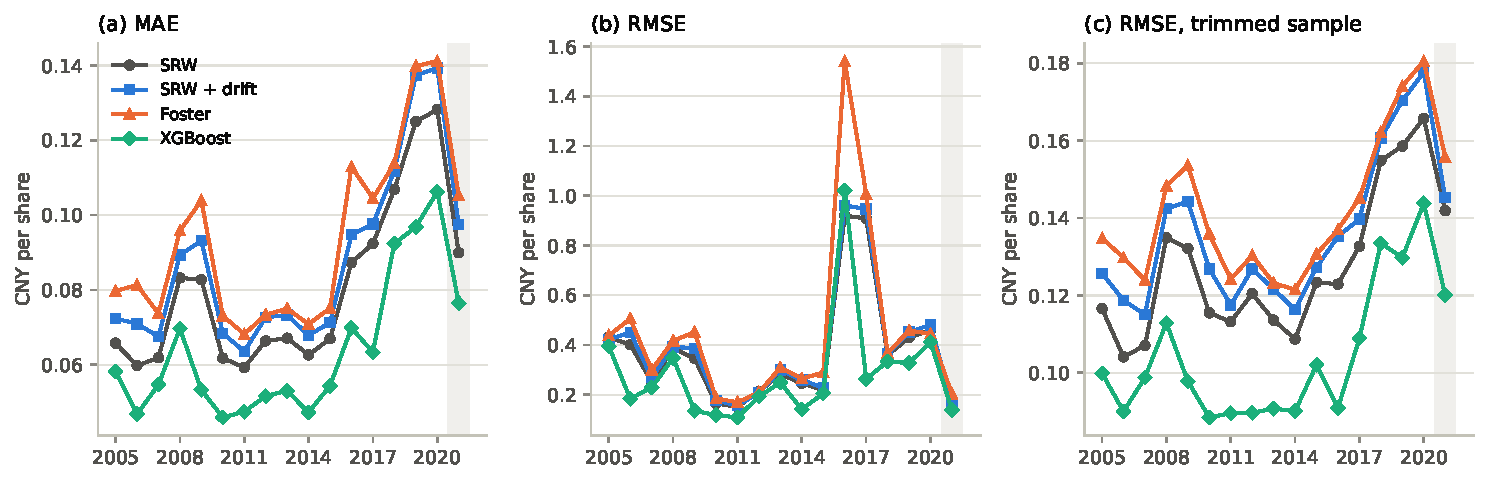
\includegraphics[width=\textwidth]{fig1_annual_accuracy.pdf}
\caption{Annual forecast accuracy on the common sample (CNY per share), by target fiscal year. Panel (c) uses the
symmetrically trimmed sample. The shaded year 2021 contains Q1 targets only.}
\label{fig:annual}
\end{figure}

\begin{figure}[!htbp]
\centering
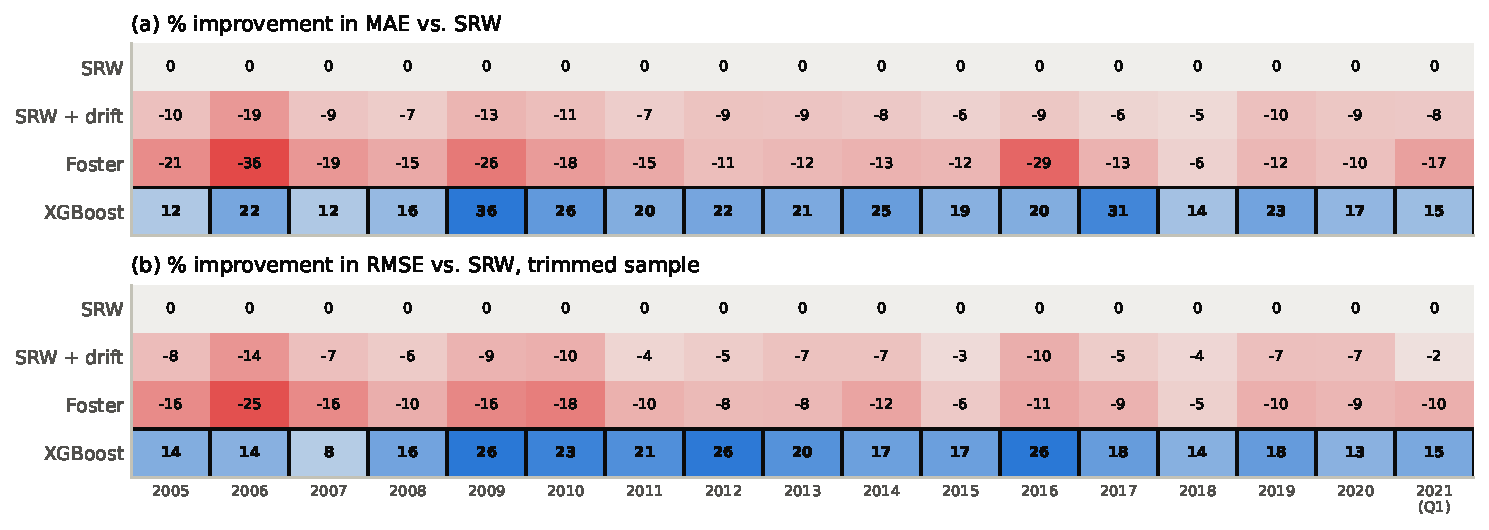
\includegraphics[width=\textwidth]{fig3_best_model_by_year.pdf}
\caption{Percentage improvement over the SRW by fiscal year (blue = better, red = worse). The outlined, bold cell is
the best model in each year. (a) MAE, common sample; (b) RMSE, trimmed sample.}
\label{fig:heat}
\end{figure}

\begin{table}[!htbp]
\centering\footnotesize
\caption{Annual accuracy. SRW columns are MAE/RMSE in CNY per share; model columns are $\%\Delta$ vs.\ SRW. Stars on
$\%\Delta$MAE use firm-clustered standard errors within the year. XGB$^{\text{trim}}$: RMSE improvement on the trimmed
sample.}
\label{tab:annual}
\resizebox{\textwidth}{!}{\begin{tabular}{lrr rrr r rrr r ll}
\toprule
& & \multicolumn{4}{c}{MAE} & \multicolumn{5}{c}{RMSE} & \multicolumn{2}{c}{Best model} \\
\cmidrule(lr){3-6}\cmidrule(lr){7-11}\cmidrule(lr){12-13}
FY & N & SRW & Drift & Foster & XGB & SRW & Drift & Foster & XGB & XGB$^{\text{trim}}$ & MAE & RMSE \\
\midrule
2005 & 2,282 & 0.0658 & $-$10.0*** & $-$21.2*** & 11.6*** & 0.4311 & 2.0 & $-$1.6 & 8.5 & 14.3 & XGBoost & XGBoost \\
2006 & 3,101 & 0.0598 & $-$18.7*** & $-$36.1*** & 21.7** & 0.4011 & $-$12.2 & $-$26.0 & 54.2 & 13.6 & XGBoost & XGBoost \\
2007 & 3,577 & 0.0619 & $-$9.2*** & $-$19.1*** & 11.6*** & 0.2522 & $-$6.6 & $-$18.8 & 9.3 & 7.7 & XGBoost & XGBoost \\
2008 & 4,001 & 0.0832 & $-$7.3*** & $-$15.1*** & 16.3*** & 0.3857 & $-$1.7 & $-$8.1 & 9.8 & 16.3 & XGBoost & XGBoost \\
2009 & 4,105 & 0.0827 & $-$12.6*** & $-$25.6*** & 35.6*** & 0.3461 & $-$11.8 & $-$30.4 & 61.0 & 26.0 & XGBoost & XGBoost \\
2010 & 4,552 & 0.0618 & $-$10.7*** & $-$18.3*** & 25.7*** & 0.1648 & $-$6.9 & $-$12.3 & 28.2 & 23.4 & XGBoost & XGBoost \\
2011 & 5,016 & 0.0593 & $-$7.2*** & $-$15.1*** & 19.9*** & 0.1514 & $-$4.1 & $-$12.0 & 28.2 & 20.9 & XGBoost & XGBoost \\
2012 & 5,200 & 0.0664 & $-$9.5*** & $-$10.5*** & 22.2*** & 0.2129 & 2.8 & 1.9 & 9.5 & 25.5 & XGBoost & XGBoost \\
2013 & 5,806 & 0.0671 & $-$9.3*** & $-$11.8*** & 21.0*** & 0.2825 & $-$6.1 & $-$9.4 & 11.7 & 20.1 & XGBoost & XGBoost \\
2014 & 6,791 & 0.0626 & $-$8.3*** & $-$13.1*** & 24.6*** & 0.2464 & $-$5.1 & $-$7.5 & 42.8 & 17.1 & XGBoost & XGBoost \\
2015 & 7,510 & 0.0670 & $-$6.4*** & $-$12.2*** & 18.8*** & 0.2182 & $-$4.5 & $-$32.7 & 5.8 & 17.3 & XGBoost & XGBoost \\
2016 & 7,816 & 0.0873 & $-$8.5*** & $-$29.3* & 20.0*** & 0.9198 & $-$4.5 & $-$67.6 & $-$11.1 & 26.0 & XGBoost & SRW \\
2017 & 7,994 & 0.0923 & $-$5.7*** & $-$13.1*** & 31.4** & 0.9089 & $-$4.2 & $-$10.8 & 71.0 & 17.9 & XGBoost & XGBoost \\
2018 & 8,512 & 0.1069 & $-$4.6*** & $-$6.5*** & 13.6*** & 0.3592 & $-$1.5 & $-$2.2 & 7.1 & 13.8 & XGBoost & XGBoost \\
2019 & 9,023 & 0.1250 & $-$9.9*** & $-$11.9*** & 22.5*** & 0.4297 & $-$5.1 & $-$6.6 & 23.8 & 18.2 & XGBoost & XGBoost \\
2020 & 9,606 & 0.1282 & $-$8.7*** & $-$10.1*** & 17.1*** & 0.4593 & $-$4.7 & 3.1 & 10.2 & 13.3 & XGBoost & XGBoost \\
2021 (Q1) & 840 & 0.0899 & $-$8.4*** & $-$17.1*** & 14.9*** & 0.1618 & $-$2.7 & $-$25.4 & 15.1 & 15.4 & XGBoost & XGBoost \\
\bottomrule
\end{tabular}
}
\end{table}

\section{Firm-level heterogeneity}

\paragraph{Error size in context.} On the untrimmed common sample, XGBoost's MAE is
0.0681 CNY per share, against 0.0860 for the SRW. Total absolute error divided by
total absolute realized EPS is 65.1\% for XGBoost and
82.2\% for the SRW. This is an aggregate ratio, not the average observation's
percentage error. Using each observation's historical EPS scale instead, the mean absolute scaled error is
98.4\% versus 114.4\%; the median is
40.1\% versus 44.9\%.
The historical scale is the mean absolute EPS known before the announcement within the preceding eight fiscal
quarters, floored at 0.01 CNY per share. Direct percentage errors relative to actual EPS are unsuitable here:
980 observations have zero EPS, and near-zero EPS makes such ratios unstable.
Thus XGBoost improves materially on the benchmark, but the remaining errors are large relative to earnings.
Forecast accuracy alone does not establish an improvement in investment returns or in the measurement of market expectations.


Firm-level comparisons use the \NFirmsFL{} firms with at least 12 common-sample forecasts (three years).
Table~\ref{tab:firm} and Figures~\ref{fig:firmhist}--\ref{fig:conc} show that XGBoost's gain is broad-based. It
beats the SRW for \FirmBetterxgb\% of firms by MAE (\FirmBetterRMSExgb\% by RMSE), and the median firm-level
improvement is \FirmMedxgb\%. Sign tests reject equal proportions for all three models. Drift and Foster beat the SRW for
only \FirmBetterrwd\% and \FirmBetterfoster\% of firms. The aggregate result is not driven by a few firms. Excluding
the 5\% of firms that contribute most to XGBoost's MAE reduction still leaves a \ExclTopFivexgb\% improvement, and
excluding the 5\% hardest-to-forecast firms leaves \ExclHardxgb\%. The concentration curve in
Figure~\ref{fig:conc}(b) rises smoothly for XGBoost, while drift and Foster lose accuracy across most of the
cross-section.

\begin{table}[!htbp]
\centering\small
\caption{Firm-level accuracy (firms with $\geq$12 common-sample forecasts). Firm $\%\Delta$MAE compares each model
with the SRW on that firm's forecasts. The last two columns re-compute the pooled $\%\Delta$MAE after excluding the
5\% of firms with the largest contribution to the model's MAE reduction, or the 5\% of firms with the highest SRW MAE.}
\label{tab:firm}
\resizebox{\textwidth}{!}{\begin{tabular}{lrrr rr rr rr}
\toprule
& \multicolumn{3}{c}{Firm-level MAE} & \multicolumn{2}{c}{Firm \%$\Delta$MAE} & \multicolumn{2}{c}{\% firms beating SRW} & \multicolumn{2}{c}{Pooled \%$\Delta$MAE excl.} \\
\cmidrule(lr){2-4}\cmidrule(lr){5-6}\cmidrule(lr){7-8}\cmidrule(lr){9-10}
Model & p10 & p50 & p90 & median & IQR & MAE & RMSE & top-5\% contrib. & 5\% hardest \\
\midrule
SRW & 0.0205 & 0.0566 & 0.1664 & -- & -- & -- & -- & -- & -- \\
SRW + drift & 0.0209 & 0.0605 & 0.1836 & $-$7.1 & [$-$11.9, $-$2.3] & 17.7 & 15.9 & $-$9.8 & $-$8.0 \\
Foster & 0.0208 & 0.0618 & 0.1908 & $-$10.6 & [$-$17.9, $-$2.0] & 21.3 & 21.6 & $-$17.6 & $-$12.0 \\
XGBoost & 0.0177 & 0.0472 & 0.1299 & 18.7 & [8.6, 27.2] & 87.7 & 86.8 & 18.2 & 19.8 \\
\bottomrule
\end{tabular}
}
\end{table}

\begin{figure}[!htbp]
\centering
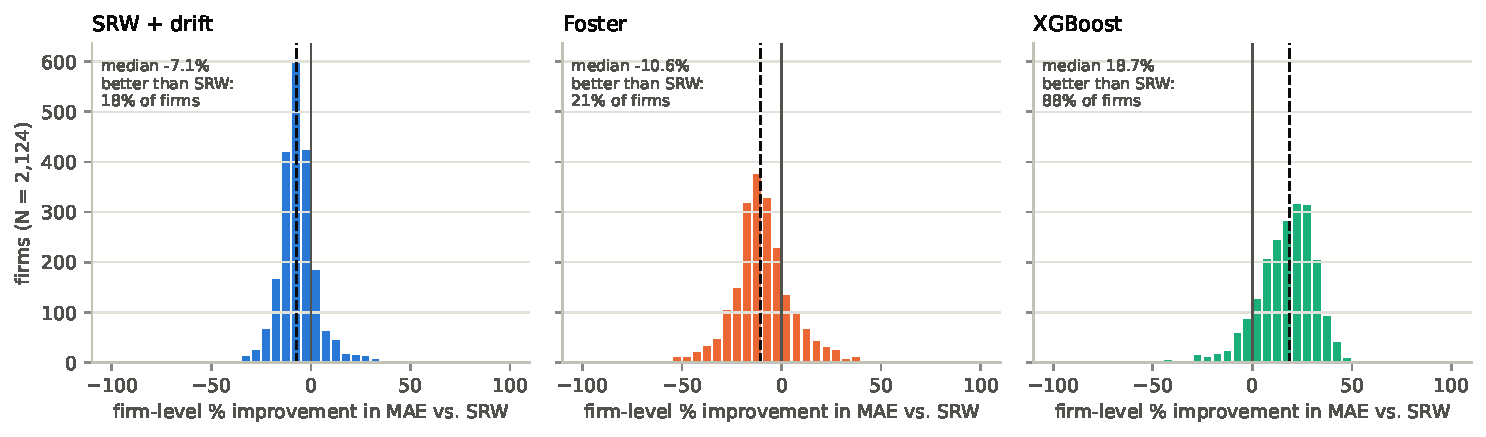
\includegraphics[width=\textwidth]{fig5_firm_improvement_hist.pdf}
\caption{Distribution of firm-level percentage MAE improvement over the SRW (values clipped to $\pm100\%$; dashed line:
median).}
\label{fig:firmhist}
\end{figure}

\begin{figure}[!htbp]
\centering
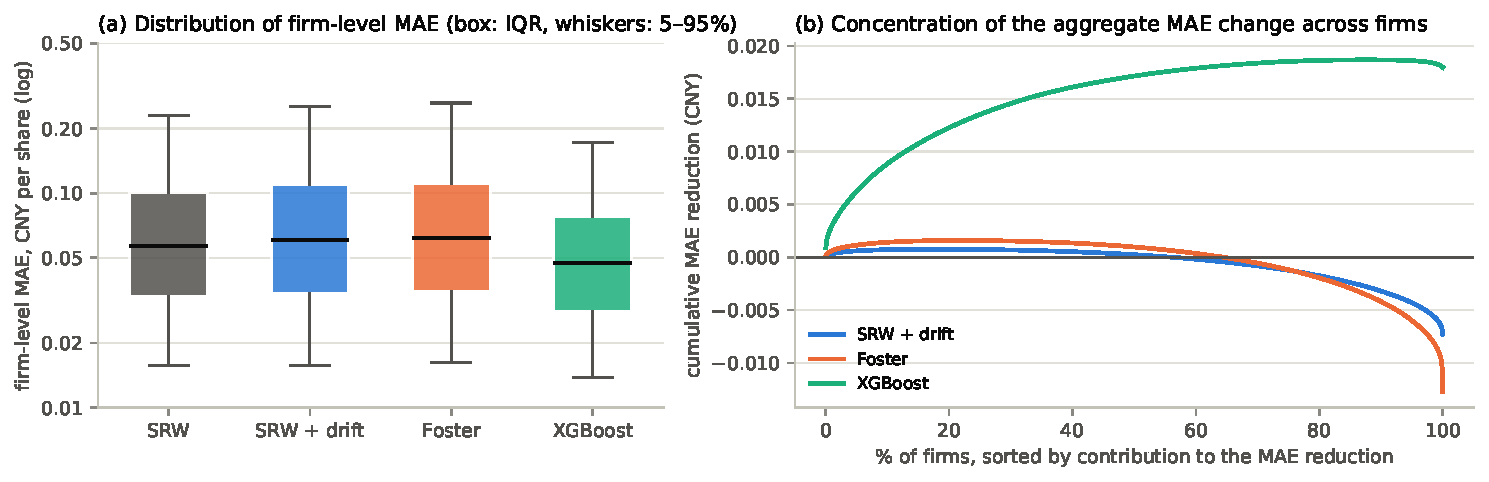
\includegraphics[width=\textwidth]{fig6_firm_distribution_concentration.pdf}
\caption{(a) Firm-level MAE by model. (b) Cumulative contribution of firms, sorted by their contribution, to the
aggregate MAE reduction relative to the SRW (end point = aggregate MAE change).}
\label{fig:conc}
\end{figure}

\paragraph{Actual and predicted EPS for selected firms.} Figures~\ref{fig:examples-best}--\ref{fig:examples-random}
plot realized quarterly EPS and the four out-of-sample forecasts. ``Best'' and ``worst'' mean the largest and smallest
firm-level percentage MAE improvement of XGBoost over the SRW, among firms with at least 12 common-sample forecasts;
they do not rank firms by their absolute forecast errors. The four random firms are sampled without replacement
from the remaining eligible firms using seed 42. All plotted observations belong to the untrimmed common sample.
The horizontal axis is the target fiscal quarter, not the announcement date; missing quarters appear as gaps.
Each firm has its own vertical scale, shared by actual EPS and all four models, with no clipping of extreme values.
The extreme examples are selected using realized forecast performance and illustrate heterogeneity rather than
providing an independent test of predictability.

\begin{figure}[p]
\centering
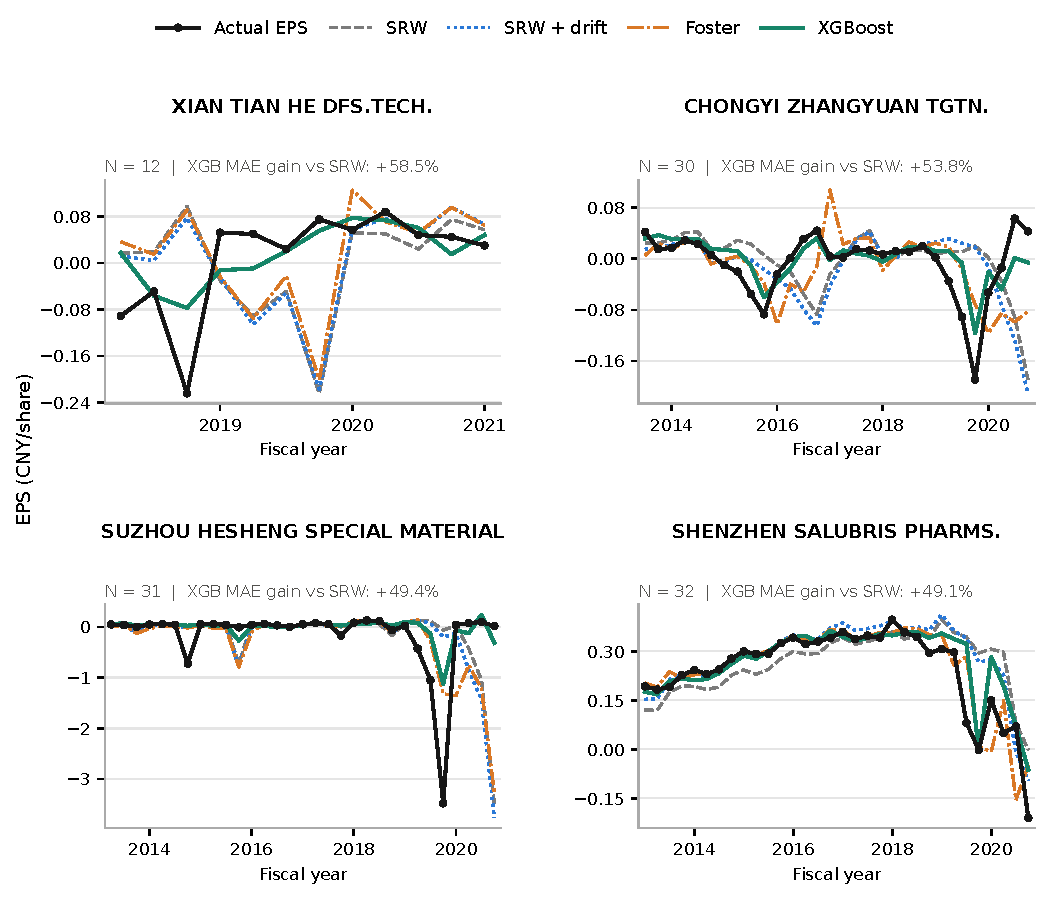
\includegraphics[width=\textwidth]{fig_firm_forecasts_best.pdf}
\caption{Actual and predicted quarterly EPS: the four firms with the largest percentage MAE improvement of
XGBoost over the SRW. Each subplot shows the firm's common-sample observation count and MAE improvement;
a positive improvement means XGBoost is more accurate.}
\label{fig:examples-best}
\end{figure}

\begin{figure}[p]
\centering
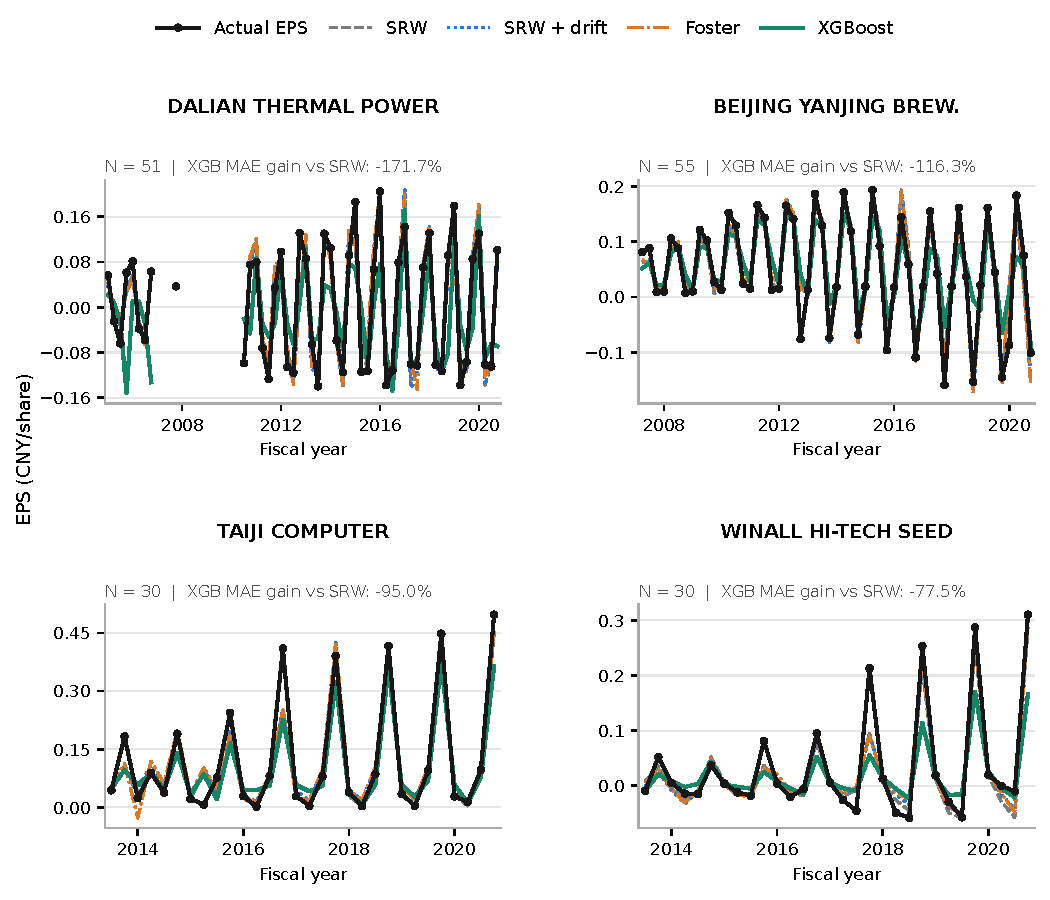
\includegraphics[width=\textwidth]{fig_firm_forecasts_worst.pdf}
\caption{Actual and predicted quarterly EPS: the four firms with the smallest percentage MAE improvement of
XGBoost over the SRW. Negative improvements indicate that XGBoost has higher MAE than the SRW.}
\label{fig:examples-worst}
\end{figure}

\begin{figure}[p]
\centering
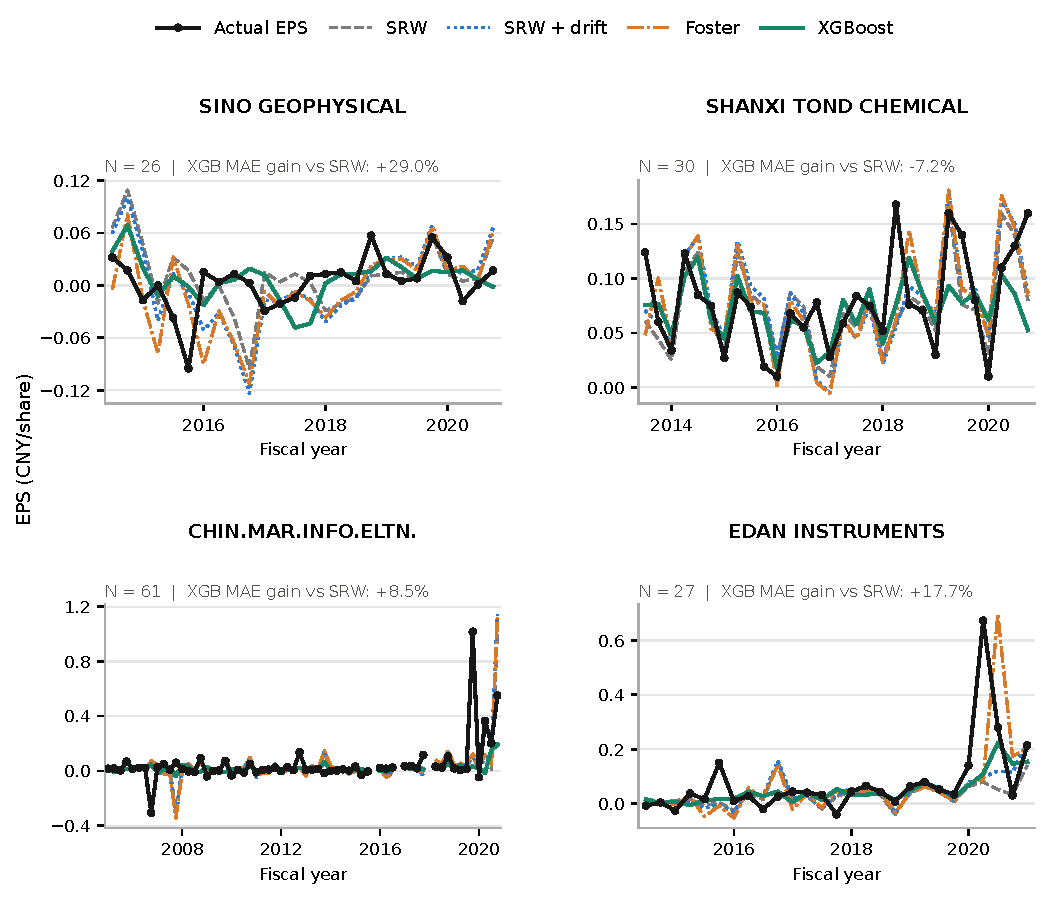
\includegraphics[width=\textwidth]{fig_firm_forecasts_random.pdf}
\caption{Actual and predicted quarterly EPS: four randomly selected firms from the eligible sample after excluding
the eight extreme examples (seed 42). Selection is unrelated to these firms' forecast ranking within that remaining sample.}
\label{fig:examples-random}
\end{figure}

\section{Discussion and conclusion}

Among the four models, only the pooled XGBoost model improves on the seasonal random walk. The gain is economically
meaningful: about a fifth of the SRW's absolute forecast error, with a lower average absolute error in
\QbetterMAExgb\% of fiscal quarters. It is stable over 2005--2021 and spread across the large majority of firms. It does not come from model complexity per se.
The two classical refinements, drift and Foster's autoregression, \emph{reduce} accuracy, because 12-quarter
firm-level histories cannot estimate weakly persistent dynamics precisely. XGBoost instead pools information across
all firms. It also learns non-linear patterns that firm-level linear models cannot represent. The most important
feature is a loss at $q-4$ (\TopImpShare\% of total gain), followed by the seasonal lag $EPS_{q-4}$, the fiscal quarter,
and the most recent YoY change. This points to strong reversal of losses, plausibly linked to Chinese delisting and
special-treatment rules for loss firms, and to quarter-specific mean reversion that the SRW ignores.

For constructing alternative SUE measures, three implications follow.
\begin{enumerate}
\item $UE^{(\text{XGB})}$ is a statistically better proxy for the unpredictable part of earnings than the SRW surprise.
A drift- or Foster-based SUE is not recommended for this sample.
\item Because the forecast is more accurate, $UE^{(\text{XGB})}$ is smaller in magnitude, and its scaling ($\sigma_i(UE)$)
must be re-estimated from the model's own historical errors rather than taken from the SRW.
\item A more accurate forecast is not necessarily the market's expectation \citep{campbell2026}. Whether PEAD and
streak effects strengthen or weaken under $UE^{(\text{XGB})}$ is itself informative: a stronger drift would indicate
that investors anchor on naive seasonal comparisons.
\end{enumerate}

The analysis has limitations:
\begin{itemize}
\item EPS is adjusted retroactively for capital changes and may contain later restatements.
\item Pre-2004 dates are backfilled, which conservatively shrinks early training data.
\item Same-day Q4/Q1 releases shorten the effective information set for a rising share of Q1 targets.
\item The XGBoost grid is intentionally small; a richer model could change its accuracy but would not change the
leakage-free design.
\end{itemize}

\begin{thebibliography}{99}
\bibitem[Bernard and Thomas(1990)]{bernard1990} Bernard, V.~L. and J.~K. Thomas (1990). Evidence that stock prices do
not fully reflect the implications of current earnings for future earnings. \emph{Journal of Accounting and Economics}
13(4), 305--340. \url{https://doi.org/10.1016/0165-4101(90)90008-R}
\bibitem[Cameron et~al.(2011)]{cameron2011} Cameron, A.~C., J.~B. Gelbach, and D.~L. Miller (2011). Robust inference
with multiway clustering. \emph{Journal of Business \& Economic Statistics} 29(2), 238--249.
\bibitem[Campbell et~al.(2026)]{campbell2026} Campbell et al. (2026). Expectations matter: When (not) to use machine
learning earnings forecasts. \emph{Management Science}. \url{https://doi.org/10.1287/mnsc.2024.05808}
\bibitem[Chen and Guestrin(2016)]{chen2016} Chen, T. and C. Guestrin (2016). XGBoost: A scalable tree boosting system.
\emph{Proceedings of the 22nd ACM SIGKDD International Conference on Knowledge Discovery and Data Mining}, 785--794.
\bibitem[Diebold and Mariano(1995)]{diebold1995} Diebold, F.~X. and R.~S. Mariano (1995). Comparing predictive
accuracy. \emph{Journal of Business \& Economic Statistics} 13(3), 253--263.
\bibitem[Foster(1977)]{foster1977} Foster, G. (1977). Quarterly accounting data: Time-series properties and
predictive-ability results. \emph{The Accounting Review} 52(1), 1--21.
\bibitem[Newey and West(1987)]{newey1987} Newey, W.~K. and K.~D. West (1987). A simple, positive semi-definite,
heteroskedasticity and autocorrelation consistent covariance matrix. \emph{Econometrica} 55(3), 703--708.
\bibitem[Pagach and Warr(2020)]{pagach2020} Pagach, D. and R. Warr (2020). Analysts versus time-series forecasts of
quarterly earnings: A maintained hypothesis revisited. \emph{Advances in Accounting} 51, 100497.
\url{https://doi.org/10.1016/j.adiac.2020.100497}
\bibitem[Thompson(2011)]{thompson2011} Thompson, S.~B. (2011). Simple formulas for standard errors that cluster by
both firm and time. \emph{Journal of Financial Economics} 99(1), 1--10.
\bibitem[Zhang et~al.(2025)]{zhang2025} Zhang, Zhu, and Linnainmaa (2025). Man versus machine learning revisited.
\emph{Review of Financial Studies}. \url{https://doi.org/10.1093/rfs/hhaf066}
\end{thebibliography}

\end{document}
